\section{Crowdsourcing Platforms}\label{sec:cloud:crowdsourcing}
\newcommand{\campaignIAT}{\ensuremath{t_c}\xspace}
\newcommand{\campaignSize}{\ensuremath{\Theta}\xspace}
\newcommand{\taskDuration}{\ensuremath{B}\xspace}
\newcommand{\meanTaskLength}{\ensuremath{E[B]}\xspace}
\newcommand{\numberOfWorkers}{\ensuremath{c}\xspace}
\newcommand{\workerUtilization}{\ensuremath{\rho}\xspace}
\newcommand{\campaignDuration}{\ensuremath{\delta}\xspace}
\newcommand{\preTaskProcessingDelay}{\ensuremath{E[D]}\xspace}
While the last sections dealt with dimensioning of systems in machine cloud systems, similar methodologies are applicable to crowdsourcing, or human clouds.
Here, a crowdsourcing platform operator enables employers to distribute microtasks to workers.
In order to ensure the success of the plattform, the operator has to ensure the satisfaction of both the employers, as they provide the main source of income, as well as the workers, the resource of the plattform.
This trade-off between employer satisfaction, i.e. time required before submitted tasks are completed, and worker satisfaction, i.e. income, has to be managed by the platform operator by carefully considering the number of workers employed at the platform.

To this end, in \refsec{sec:cloud:crowdsourcing:model} we first provide a mode for crowdsourcing plattforms regarding the two identified metrics.
Then, we study parameters of a real world crowdsourcing platform in \refsec{sec:cloud:crowdsourcing:measurements}.
Finally, in \refsec{sec:cloud:crowdsourcing:performance_evaluation} we evaluate the provided model using the obtained parameters and discuss the trade-off between employer and worker satisfaction from the point of view of the plattform operator.

\subsection{Models of \headershortacr{GGSN} Implementations}\label{sec:cloud:virtualized_network_functions:model}

In this section we provide a model for a traditional \gls{GGSN} and discuss a model for a virtual \gls{GGSN} using \gls{NFV}.
In \gls{NFV} \cite{Nfv2013} static network middleboxes are replaced by commodity hardware.
The tasks solved by the original middleboxes are then solved by dedicated software.

\subsubsection*{Traditional GGSN}\label{sec:cloud:virtualized_network_functions:model:traditional_ggsn}
First, we give a model for a \emph{traditional} \gls{GGSN}, i.e. a static network component.
While we consider the \gls{GGSN} to be one fixed entity, it can in reality consist of multiple servers.
However, due to the fact that the \gls{GGSN} is purchased from a vendor as a middlebox, idle servers can be neither deactivated nor reused for other purposes.

\begin{figure}
  \centering
  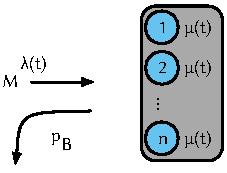
\includegraphics{cloud/virtualized_network_functions/model/figures/traditional_ggsn}
  \caption{Considered model of a traditional \headershortacr{GGSN}.}
  \label{sec:cloud:virtualized_network_functions:model:traditional_ggsn:model}
\end{figure}

We present an abstract queueing model for the traditional \gls{GGSN} in \reffig{sec:cloud:virtualized_network_functions:model:traditional_ggsn:model}.
New tunnels requests arrive according to a Poisson process with rate \(\lambda(t)\) at the \gls{GGSN}.
This server will support a maximum tunnel capacity of \(c\).
When this capacity is reached, blocking will occur and newly incoming tunnels requests are rejected.
Traditionally, \glspl{GGSN} can be expected to be overdimensioned in such a way that this rarely happens.
If the new tunnel is accepted, it will occupy one of the serving units of the server for the duration \(\mu(t)\) of the tunnel.
As stated earlier, we can not model the tunnel duration to be markovian, resulting in a  \(M/GI/c\) loss system.
In order to give quality of service guarantees the network operator is interested in the system's blocking probability \(\blockingprobability\), which we consider to be a key metric of our model.
Additionally, the previously described diurnal patterns can also be modelled by adjusting the arrival and serving process distributions for each time of day.
This alternatively also allows just to investigate the busy hour and thus the system's peak load.

\subsubsection*{\headershortacr{GGSN} using Network Function Virtualisation}\label{sec:cloud:virtualized_network_functions:model:virtual_ggsn}
Next, we introduce concepts from \gls{NFV}, i.e. the idea to replace middleboxes with commodity hardware as an extended model in \reffig{sec:cloud:virtualized_network_functions:model:virtual_ggsn:model}.
This allows us to realise benefits from cloud computing, as we are now able to scale out, instead of up.
The assumptions of the Markov arrival process \(\lambda(t)\) and the serving time distributions \(\mu(t)\) are carried over.
However, instead of one server processing every tunnel, this model assumes that there are up to \(s_{max}\) virtualised servers \(s_i\).
Each of these is less powerful than the traditional \gls{GGSN}, having a tunnel serving capacity of \(c_i \ll c\) and a total system capacity of \(c_{max} = s_{max} \times i\).

\begin{figure}
  \centering
  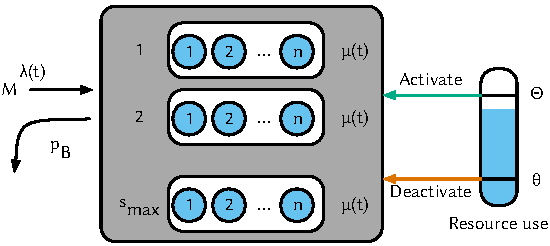
\includegraphics{cloud/virtualized_network_functions/model/figures/virtual_ggsn}
  \caption{Considered model of a virtualised \headershortacr{GGSN}.}
  \label{sec:cloud:virtualized_network_functions:model:virtual_ggsn:model}
\end{figure}

In its initial state, for efficiency, all but a small portion of the server instances are considered to be disabled.
Only, when a certain condition is reached, a new server instance is provisioned.
As a simple example, one instance could be kept in reserve for upcoming requests and an additional would be provisioned as soon as the reserve is used.
Similar rules should apply in the shut-down of servers and form a hysteresis with the boot condition.
For example it would be possible to keep at least one server in reserve but never more than two.

If these conditions are not carefully selected and are in tune with the expected boot time of an instance, additional blocking can occur.
Despite not having reached its maximum capacity, this system would still reject tunnel requests during the provisioning phase when no tunnel slots are available.
This could be remedied by a request queue.
However, this would introduce additional complexity to the system without providing real benefit, as mobile devices or applications will repeat their attempts and would timeout when the request is taking too long.

To place incoming tunnel state on one of the available servers a load balancer is required.
To ensure that the system in run time can scale down to its actual needs, the balancer should place tunnels on servers that are the fullest, keeping the reserve free.
It may even migrate tunnel state from almost empty servers away so that these can be shut down, when the shut-down condition is fulfilled.
Keeping instance close to their capacity should also have no impact on the performance a mobile device associated to a specific tunnel experiences.

\subsection{Measurements}\label{sec:cloud:crowdsourcing:measurements}
In this section we analyse a large dataset from a commercial crowdsourcing platform to derive to derive realistic model parameters and compare the model based on these results with the analytic approximation.

\subsubsection*{Deriving Realistic Model Parameters}
Our analysis is based on a large dataset from the commercial micro-tasking platform Microworkers.com.
The dataset contains information about more then 160.000 campaigns submitted to the platform between May 2009 and Jan 2015, including the number of task per campaign was well as the time of the submission of the campaign.  

\paragraph*{Interarrival Times:} First, we study the inter-arrival times of the campaigns.
During the observation period, the platform faced some downtime due to software update or changes of the technical infrastructure.
During this time, no campaigns could be submitted resulting in relatively large campaign inter-arrival times.
In our model we only consider the regular operation of the platform, therefore we removed all inter-arrival times larger then \SI{97.5}{\percent} quantile of all observed values, which affects about \SI{2.5}{\percent} of all values.

\begin{figure}
  \centering
  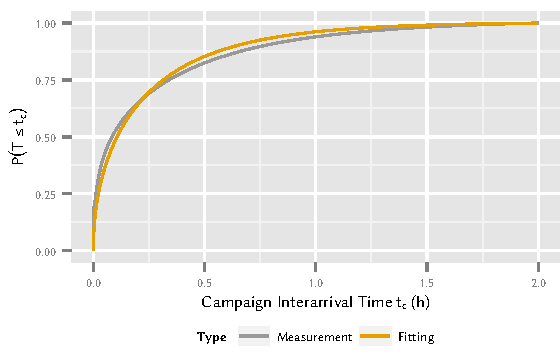
\includegraphics{cloud/crowdsourcing/measurements/figures/campaign_interarrival}
  \caption{Observed campaign inter-arrival times \(t_c\) and corresponding fit.}
  \label{fig:cloud:crowdsourcing:measurements:parameters:campaign_interarrival}
\end{figure}

Considering the remaining data, we observe a mean campaign inter-arrival time of \SI{0.241}{\hour} with a standard deviation \SI{0.346}{\hour}.
\reffig{fig:cloud:crowdsourcing:measurements:parameters:campaign_interarrival} shows the \gls{CDF} of considered inter-arrival times, as well as the fitted distribution.
For the fitting we considered several possible distributions but found the Gamma-distribution 

\[
P(t_c=t) \sim \Gamma(\alpha,\beta,t_c) = \frac{\beta^\alpha}{\Gamma(\alpha)} x^{\alpha-1} e^{-{\beta}t_c}
\]

defined by shape \(\alpha\) and rate \(\beta\) to be the most suitable.
Using \texttt{fitdistrplus} for the R language we derive the distribution parameters by moment fitting and result in the estimated parameters \(\alpha=0.484\) and \(\beta=2.009\).

\paragraph*{Campaign Sizes:}Next, we consider the campaign sizes, respectively the number of tasks per campaign.
The smallest possible campaign sizes on Microworkers is \(30\) tasks, however our dataset contained a few internal test campaigns with a small size.

These test campaigns, as well as outliers larger than the \SI{97.5}{\percent} quantile of the campaign size have been removed from the considered dataset.
In total \SI{3.7}{\percent} of the original dataset were filtered by these conditions, the remaining data resulted in a mean campaign size of \(97.01\) tasks and a standard deviation of \(103.41\).
The CDF of the campaign sizes is depicted in \reffig{fig:cloud:crowdsourcing:measurements:parameters:campaign_sizes}, together with the corresponding fitted distribution.

\begin{figure}
  \centering
  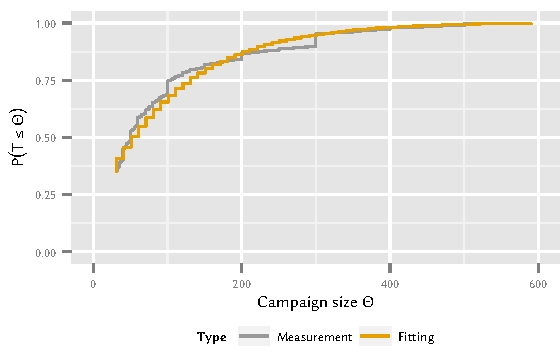
\includegraphics{cloud/crowdsourcing/measurements/figures/campaign_sizes}
  \caption{Observed campaign sizes \campaignSize and corresponding fit.}
  \label{fig:cloud:crowdsourcing:measurements:parameters:campaign_sizes}
\end{figure}

Due to the platform restrictions mentioned above, the campaign sizes start with a minimum value of \(30\) tasks.
We observer that a very high share, i.e. \SI{35}{\percent}, of campaigns has only this minimum size.
Further, campaign sizes which are a multiple of ten or a multiple of \(100\) are quite frequent.
This is caused by the fact that most task on Microworkers.com are repetitive and the employers choose the required number of repetitions and thus are more likely to round the number of repetitions to the nearest multiple of ten or \(100\).

In order to obtain an suitable analytic distribution for the empiric values, we divided the observed values and use the following piecewise defined distribution.
\begin{equation*}
P(S=s) \sim
\begin{cases}
  0 & \text{if } s < s_{\min}\\
  p_{s_{\min}} & \text{if } s=s_{\min} \\
  GEOM(s) \cdot 10 + (s_{\min}+1) & \text{else}
\end{cases}
\end{equation*}
with 
\begin{equation*}
GEOM(s) = {(1-p)}^s p
\end{equation*}
The minimum campaign size \(s_{\min}\) is observed with a fixed probability \(p_{s_{\min}}\), while all campaign sizes larger then \(s_{\min}\) follow a shifted and scaled geometric distribution.

Due to the relatively high frequencies of campaign sizes being multiples of \(10\) and \(100\), it is only possible to achieve a good fitting either for the lower or the higher region of the geometric part.
As an overestimation of the campaign size will give us an upper bound of the platform work load, we decided to put a stronger emphasis on correct fitting of the larger campaign sizes.

Using the \texttt{fitdistrplus} package for the R language we estimate the \(p=0.086\) parameter of the geometric distribution using quantile matching for the \SI{90}{percent} quantile.
The values \(s_{\min}=30\) and \(p_{s_{\min}}=0.350\) are obtained from the empirical values.

\paragraph*{Task Duration: }Another relevant model parameter is the processing time of the tasks, i.e., the time a single worker needs to complete one tasks.
Unfortunately, this information cannot be obtained from our dataset, as tracking of the individual workers is not possible.
Therefore, we assume that the processing times follow a negative-exponential distribution, i.e.
\begin{equation*}
P(t_p=t) \sim \mu  e^{-{\mu}t}
\end{equation*}
Even if the exact processing times are not available, each employer has to add an estimation about the time it task to complete a task in the campaign description.
In our dataset, \SI{87.8}{\percent} of all tasks had an estimated completion time between \SIrange{60}{300}{\second}.
Therefore, we consider \(\mu \in \{\frac{1}{6},\frac{1}{5},\hdots,\frac{1}{2},1\}\) for the following evaluations.

\paragraph*{Number of Workers: }Finally, the last model parameter to estimate is the number of users on the crowdsourcing platform. 
At the time of this analysis, Microworkers.com had over 650.000 registered user accounts.
However, this number is not applicable in the proposed model, for multiple reasons.
The proposed model does not consider vacation times, i.e., the workers would have to be available 24/7.
In reality, many crowdsourcing workers only work occasionally on the platforms or only for a few tasks.
Further, employers can limit the access of to their campaigns to specific subset of all workers, which is also not considered in the model.
Moreover, Microworkers also limits the number of tasks a worker can complete in a single campaign.
Taking this into account, the number of workers to be considered in our model has to be much small then the number of workers on the real world platform and consequently we decided to estimate meaningful values based on the model parameters instead of using the given number of workers from the dataset.

\subsubsection*{Comparison of Detailed and Analytical Model}
An important question for the later analysis is whether the analytic model from \refsec{sec:cloud:crowdsourcing:model} can be used as an approximation or if a simulative evaluation is necessary.
To this end we compared the later considered metrics \workerUtilization and \preTaskProcessingDelay for 
\begin{enumerate*}
\item a simulation using the empiric distributions for the task inter-arrival times and campaign sizes,
\item a simulation using the fitted distributions derived earlier in this section, and
\item the analytic model derived in \refsec{sec:cloud:crowdsourcing:model}.
\end{enumerate*}
For the analytical model we used the campaign size distribution derived in this section and \(\lambda=\SI{4.14}{\per\hour}\).
The results of the different models are shown in \reffig{fig:cloud:crowdsourcing:measurements:comparison:distribution}.

\begin{figure*}
	\centering
	\begin{subfigure}{\columnwidth}
		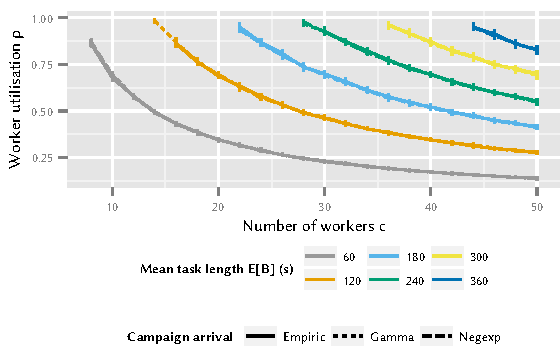
\includegraphics{cloud/crowdsourcing/measurements/figures/distribution_utilization}
		\caption{Worker utilization}
		\label{fig:cloud:crowdsourcing:measurements:comparison:distribution:utilization}
	\end{subfigure}

	\begin{subfigure}{\columnwidth}
		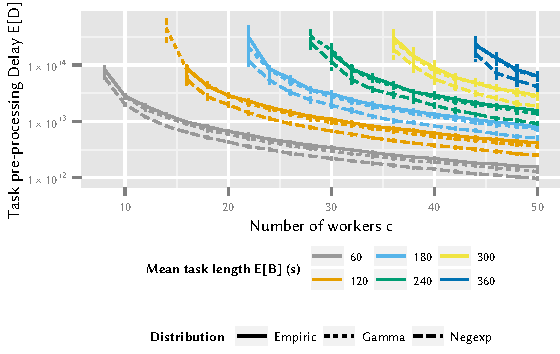
\includegraphics{cloud/crowdsourcing/measurements/figures/distribution_task_delay}
		\caption{Task pre-processing delay}
		\label{fig:cloud:crowdsourcing:measurements:comparison:distribution:task_delay}
	\end{subfigure}
	\caption{Comparison of campaign arrival distributions.}
	\label{fig:cloud:crowdsourcing:measurements:comparison:distribution}
\end{figure*}

The worker utilisation \workerUtilization is depicted in \reffig{fig:cloud:crowdsourcing:measurements:comparison:distribution:utilization}, the task pre-processing delay \preTaskProcessingDelay in \reffig{fig:cloud:crowdsourcing:measurements:comparison:distribution:task_delay}.
In both figures, the x-axis shows the number of workers \(n\).
The line colour indicates the mean task length, ranging from \SIrange{60}{360}{\second}, the line style denotes the underlying model.
We observe that all models result in the same values of \workerUtilization, which is not surprising when considering \(\workerUtilization = \frac{E[t_c] E[\campaignSize]}{c\mu}\) with the mean inter-arrival time \(E[t_c]\).
Here, all parameters are the same for the tree compared models and therefore, no significant differences can be seen.

This is different for the task pre-processing delay \preTaskProcessingDelay. 
Here, large discrepancies can been observed between the model based on the empiric distributions and the analytical model.
This results show that the \(M^{[\campaignSize]}/M/\numberOfWorkers-\infty\) model can also not be used as a worst case estimations, due to the fact that it underestimates \preTaskProcessingDelay.
In contrast to this, the simulation model based on the gamma distribution fit quite accurate the model based on the empirical values.
Therefore, we decide continue our evaluation with the simulation model, based on the gamma distributed inter-arrival times and the piecewise defined distribution for the campaign sizes.

\subsection{Numerical Evaluation}\label{sec:application:lte_video:numerical_evaluation}

In this section we study the metrics introduced in \refsec{sec:application:lte_video:system_model:model_assumptions:metrics} on the different transmission mechanisms.

First, we study the impact of the considered transmission mechanisms on the energy consumption and the wasted traffic. 
Then, we consider the impact of the connection count for the \streaming mechanisms and varying values of the parameters \emph{stop threshold} \bufferlower and \emph{threshold size} \buffersize in more detail.

We consider a video of \(\videolength=\SI{1600}{\second}\) length which is viewed on a \gls{UE} with \gls{LTE} access.
The median of available downlink throughput in current \gls{LTE} networks is \(\bandwidth = \SI{12.74}{\mega\bit\per\second}\) \cite{Huang2012}.
A wide set of video bitrates between \SIlist{1;50}{\mega\bit\per\second} is in use~\cite{YouTube2013}.
In order to prevent stalling, we consider bitrates between \SIrange{1}{10}{\mega\bit\per\second}, staying below the available network bandwidth.
For the \streaming mechanism, a stop threshold of \(\bufferlower = \SI{4}{\second}\) and a threshold size of \(\buffersize = \SI{32}{\second}\) were selected.
Furthermore, we specify a prebuffering duration of \(\streamingstart = \SI{5}{\second}\).

We conduct our study using deterministic discrete event simulation which uses no random variables.
The wasted traffic is obtained analytically using the abort behaviour model.
Thus, all results are exact under the previously stated assumptions.

\subsubsection*{Energy Consumption}\label{sec:application:lte_video:numerical_evaluation:energy_consumption}
First, we study the influence of both video bitrate as well as the selected download mechanism on energy consumption in \reffig{fig:application:lte_video:numerical_evaluation:energy_consumption:bitrate2energy}.
\begin{figure}
  \centering
  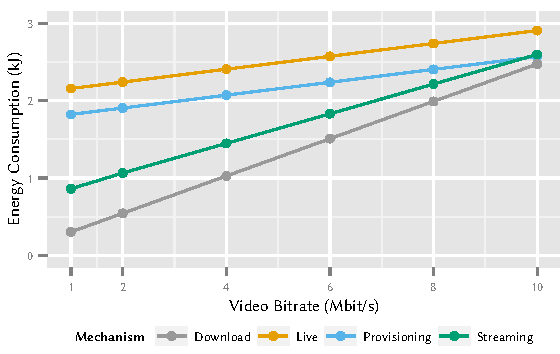
\includegraphics{application/lte_video/numerical_evaluation/figures/bitrate2energy}
  \caption{Influence of bitrate and download mechanism on energy consumption.}
  \label{fig:application:lte_video:numerical_evaluation:energy_consumption:bitrate2energy}
\end{figure}

We consider the \download mechanism and observe that it consumes the least amount of energy.
Here the video is downloaded with full bandwidth, as seen in \reffig{fig:application:lte_video:system_model:video_model}, resulting in a very short energy intensive download phase and a longer energy unintensive playback phase.
For the \live mechanism we observe the opposite, i.e. the highest energy consumption for all bandwidths.
If this mechanism is used, the used bandwidth equals the video bitrate.
Thus, the download requires the same amount of time as the playback, resulting in the highest possible energy consumption.
The \serviceprovisioning method uses a higher bandwidth, thus reducing the overall download time.
This reduced download time decreases the energy consumption when compared to the \live mechanism, even though the bandwidth used for downloading is increased to \SI{120}{\percent}.
For the \streaming mechanism we observe an energy consumption slightly higher than the \download mechanism.
As the bitrate of the video increases, the energy consumption increases as well.
This is due to the fact that a higher video bitrates require larger downloads.
For video bitrates approaching the available bandwidth the \streaming mechanism degenerates to the \live mechanism, as no prebuffering is possible.
We conclude that the \download and \streaming mechanisms outperform \live and \serviceprovisioning with regard to energy consumption.

\subsubsection*{Wasted Traffic}\label{sec:application:lte_video:numerical_evaluation:wasted_traffic}
Next, we consider the wasted traffic as a metric of the transmission mechanism quality.
If a user completely watches a video, no traffic is wasted, as all data downloaded is used during playback.
Thus, we consider only the cases where a user stops the playback before the video is finished.

\begin{figure}
  \centering
  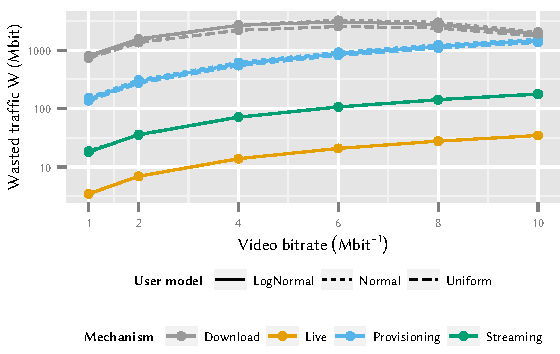
\includegraphics{application/lte_video/numerical_evaluation/figures/bitrate2lostData}
  \caption{Influence of bitrate, download mechanism and user model on wasted traffic. Download, Live, and Provisioning mechanisms result in equal connection counts.}
  \label{fig:application:lte_video:numerical_evaluation:energy_consumption:bitrate2lostData}
\end{figure}

In \reffig{fig:application:lte_video:numerical_evaluation:energy_consumption:bitrate2lostData} we study the wasted traffic for different video bitrates.
We consider the different transmission mechanisms introduced in \refsec{fig:application:lte_video:system_model:video_model} as well as the previously introduced user models.
We observe that the choice of user model has no significant impact on the wasted traffic.
For the \download mechanism, the amount of wasted traffic increases up to a video bitrate of \SI{6}{\mega\bit\per\second}, then the wasted traffic decreases as only video data which has been prebuffered can be lost if the user aborts the video.
As we assume an available bandwidth of \SI{12.74}{\mega\bit\per\second}, the bandwidth available for prebuffering decreases as the bitrate increases, resulting in lower amounts of wasted traffic for high video bitrates.
For the \live mechanism, we see that the wasted traffic for all user models is very low, but wasted traffic exists.
This is due to the traffic already sent by the server while the \gls{UE} is still waiting for promotion from \rrcidle to \rrcconnected, i.e. a short prebuffering phase exists.
As the bandwidth increases with the video bitrate, the wasted traffic increases as well.
Next, we consider the \serviceprovisioning approach and see an increase of wasted traffic as the video bitrate increases, due to the fact that the bandwidth used for continuous download is a factor of the video bitrate.
A higher video bitrate results in the download of the video being completed earlier, which leads to more wasted traffic.
Similar results can be seen for the \streaming mechanism, which results in more wasted traffic than the \live mechanism, but significantly less traffic than the \serviceprovisioning mechanism.
This is due to the fact that if the user aborts, at least the amount of video given by the \emph{stop threshold} \bufferlower and at most the complete buffer, given by the \emph{stop threshold} and the \emph{threshold size} are lost.
We have observed that the choice of user model results in no qualitative changes in wasted traffic.
As described in the last paragraph, the \download and \streaming mechanisms provide best results with regard to energy consumption.
However with regard to wasted traffic, the \live and \streaming mechanisms are most suited.
Thus, the \streaming mechanism seems to be a good compromise.
The network operator can select a tradeoff between energy consumption and wasted traffic as discussed in the next section.
From now on, we only consider the uniformly distributed user model.

\subsubsection*{Connection Count}\label{sec:application:lte_video:connection_count}
The \gls{ISP} is interested in reducing the number of connections occurring during video transmission.
Thus, we quantify the impact of the selected video transmission mechanism on the connection count, which directly correlates with the occurring signalling.

\begin{figure}
  \centering
  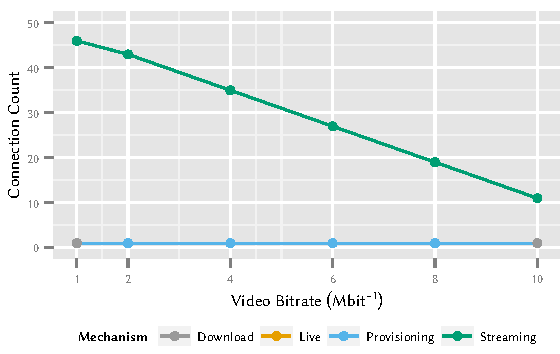
\includegraphics{application/lte_video/numerical_evaluation/figures/bitrate2connections}
  \caption{Influence of bitrate and download mechanism on connection counts.}
  \label{fig:application:lte_video:numerical_evaluation:energy_consumption:bitrate2connections}
\end{figure}

In \reffig{fig:application:lte_video:numerical_evaluation:energy_consumption:bitrate2connections} we study the impact of the different transmission mechanisms on the number of connections per transmission and thus the amount of generated signalling.
We observe that for the transmission mechanisms download, live, provisioning the number of connections is constantly one, independent of the selected bitrate \bitrate.
This is due to the fact that in these transmission mechanisms the video is transmitted in one chunk.
For streaming, the number of connections decreases as the video bitrate increases.
Here, a connection occurs each time the buffer is refilled.
For larger bitrates, refilling the buffer requires a longer transmission.
As the maximum time of video transmission is upper bounded by the video length, longer buffering phases result in a smaller total amount of buffering phases and thus in less connections per video transmission.

\begin{figure}
  \centering
  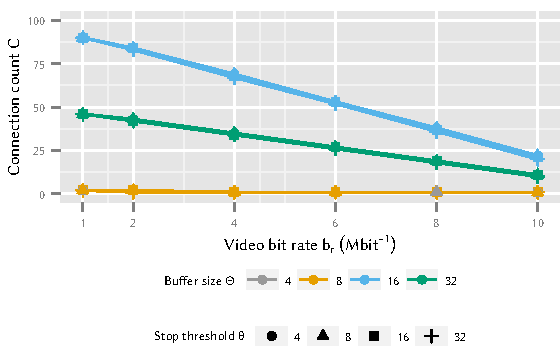
\includegraphics{application/lte_video/numerical_evaluation/figures/bitrate2connections_parameters}
  \caption{Influence of bitrate and selected parameters on connection counts for the streaming mechanism. Lines for different Stop Thresholds \(\theta\) overlap.}
  \label{fig:application:lte_video:numerical_evaluation:energy_consumption:bitrate2connections_parameters}
\end{figure}

Next, we consider the impact of the stop threshold~\bufferlower and buffer size~\buffersize on the number of connections \connectioncount caused by the \streaming mechanism.
In \reffig{fig:application:lte_video:numerical_evaluation:energy_consumption:bitrate2connections_parameters} we observe that while the buffer size has a significant impact on the number of connections during a video transmission, the lower buffer threshold has almost no impact.
For buffer sizes of \SIrange{4}{8}{\second}, no new connections are started, i.e. no signalling occurs.
This is due to the fact that the connection timeout in \gls{UE} is configured as \SI{11.576}{\second}, as discussed in \refsec{sec:application:lte_video:system_model:lte_network_model}.
Thus, for this low buffer sizes the \gls{UE} does not disconnect from the network.
Furthermore, we observe that as the buffer size increases, the number of connections decreases.
Refilling larger buffers requires, similar to larger bitrates, longer transmission times.
Thus, due to the total upper bound on the transmission time, less download phases can occur during the transmission.